
%***************************************************************************
%
% CreditCruncher - A portfolio credit risk valorator
% Copyright (C) 2004 Gerard Torrent
%
% This program is free software; you can redistribute it and/or
% modify it under the terms of the GNU General Public License
% as published by the Free Software Foundation; either version 2
% of the License.
%
% This program is distributed in the hope that it will be useful,
% but WITHOUT ANY WARRANTY; without even the implied warranty of
% MERCHANTABILITY or FITNESS FOR A PARTICULAR PURPOSE.  See the
% GNU General Public License for more details.
%
% You should have received a copy of the GNU General Public License
% along with this program; if not, write to the Free Software
% Foundation, Inc., 59 Temple Place - Suite 330, Boston, MA 02111-1307, USA.
%
%
% implementation.tex - TeX documentation file - $Rev$
% --------------------------------------------------------------------------
%
% 2005/01/22 - Gerard Torrent [gerard@fobos.generacio.com]
%   . initial release
%
% 2005/10/15 - Gerard Torrent [gerard@fobos.generacio.com]
%   . added Rev (aka LastChangedRevision) svn tag
%
%***************************************************************************

\chapter{Implementaci\'on}
\label{sec:implementation}

El m\'etodo de resoluci\'on expuesto en el cap\'itulo anterior es
computacionalmente muy costoso. Para reducir el n\'umero de operaciones
se discretiza el tiempo. Esto fuerza a mapear el recovery y el cashflow
a los nodos de tiempo. El tiempo de fallido de los clientes debe
simularse mapeado sobre los nodos. La unidad de tiempo es el mes.


\section{Paso 1. Interpretaci\'on del fichero de entrada}

El formato del fichero de entrada se encuentra descrito en el
documento \emph{CreditCruncher - Input File Reference}.
\newline
\newline
El fichero de entrada puede tener un tama\~no considerable (superior
a los 100 Mb.). Por este motivo la interpretaci\'on del fichero xml se
realiza usando un sistema orientado a eventos (tipo SAX). A continuaci\'on
se describen algunas de las validaciones m\'as importantes:

\paragraph{Formato.} Se verifica que se trata de un fichero XML
v\'alido que cumple la DTD. V\'ease \emph{W3C}\footnote{http://www.w3.org/XML/}
para m\'as informaci\'on relativa al formato XML.

\paragraph{Valores.} Cada valor tiene un tipo (int, long, double,
date, boolean o string), un rango de valores permitidos y un
indicador de obligatorio/opcional. Para cada valor se comprueba
que se cumplen los criterios descritos en
\emph{CreditCruncher - Input File Reference}.

\paragraph{Consistencia.} Cuando un valor se refiere a un identificador,
se comprueba que el objeto referenciado existe. Por ejemplo, cuando se
lee una transici\'on en la definici\'on de la matriz de transici\'on se
comprueba que los ratings han sido definidos anteriormente y que los
ratings referenciados existen.

\paragraph{Matriz de transici\'on.} Al leer la matriz de transici\'on
se verifica que cumple con las propiedades indicadas en
\ref{sec:mtransition:properties}.

\paragraph{Funci\'on de supervivencia.} En caso de estar definida
una funci\'on de supervivencia, se comprueba que se trata de una
funci\'on positiva mon\'otona decreciente que vale $1$ cuando $t=0$,
(excepto para el rating $Default$ para la que siempre vale $0$).
V\'ease las f\'ormulas \ref{prop:survival1} y \ref{prop:survival2}.

\paragraph{Matriz de correlaci\'on.} Se comprueba que se trata de
una matriz sim\'etrica (por comodidad, puede entrarse solamente
el triangulo superior, o inferior), con valores comprendidos
en $[-1,+1]$.

\paragraph{Criterios de parada.} Se comprueba que exista alg\'un
criterio de parada y que este sea realizable.

%---------------------------------------------------------------------------

\section{Paso 2. Particionamiento del tiempo}

Para realizar la discretizaci\'on del tiempo se necesita la fecha inicial, $t_0$,
la longitud (en meses naturales) de cada intervalo, $StepLength$, y el n\'umero
de pasos a considerar, $NumSteps$. Los nodos de tiempo son:
\begin{displaymath}
t_i = t_0 + i \cdot StepLength \qquad i \in \{0, 1, 2, \cdots, NumSteps\}
\end{displaymath}

Entendemos que a\~nadir $n$ meses a una fecha consiste en incrementar el
mes de la fecha inicial en $n$ meses, realizando un incremento de a\~no si
es preciso. Si el d\'ia de la fecha inicial no existe en el mes de la fecha
final, consideramos como d\'ia de la fecha final el m\'aximo d\'ia del mes
de la fecha final, en caso contrario, el mismo d\'ia de la fecha inicial.
\newline
\newline
Supongamos que $t_0=30/10/2004$, $StepLength=2$ y $NumSteps=6$, entonces la
partici\'on del tiempo es: $t_0=30/10/2004$, $t_1=30/12/2004$, $t_2=28/02/2005$,
$t_3=30/04/2005$, $t_4=30/06/2005$, $t_5=30/08/2005$ y $t_6=30/10/2005$.
Obs\'ervese como el d\'ia del mes de Febrero es el $28$ por no existir los
d\'ias $29$ y $30$ de dicho mes.

\begin{figure}[!hb]
\begin{center}
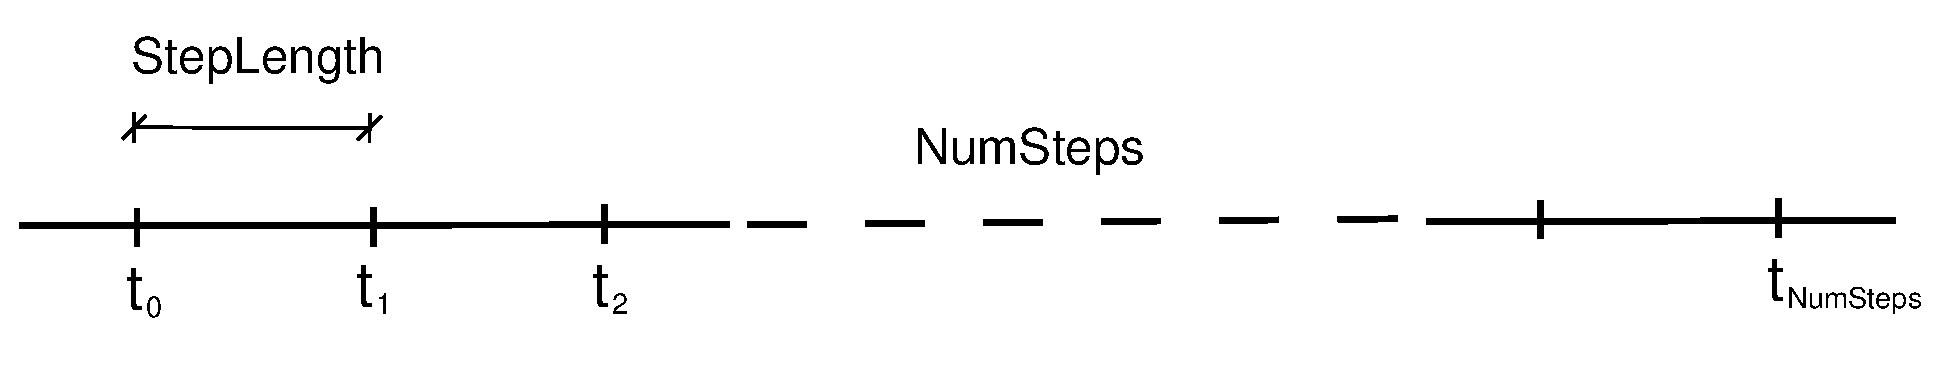
\includegraphics[width=10cm,angle=0]{./images/time.eps}
\caption{Particionamiento del tiempo}
\label{timetranches}
\end{center}
\end{figure}

%---------------------------------------------------------------------------

\section{Paso 3. Inicializaci\'on de los clientes}

Los clientes de la cartera se ordenan en funci\'on de su sector
y rating de forma creciente en ambos casos, La finalidad de esta
ordenaci\'on es disponer de una matriz de correlaci\'on entre
clientes en bloques\index{Matriz en bloques}. V\'ease las observaciones del
apartado \ref{sec:mcorrel}. Si solamente se simulan los clientes activos 
(aquellos que tienen alg\'un producto activo durante el periodo simulado)
entonces los clientes inactivos son suprimidos.
\newline
\newline
Supongamos que tenemos 3 sectores, S1, S2 y S3 y un sistema de
ratings compuesto por las clasificaciones A, B, C, D, y E.
Supongamos que la cartera est\'a compuesta por \footnote{el
primer componente corresponde al sector del cliente, el segundo al
rating del cliente y el tercero indica si est\'a activo (1) o inactivo (0)}:
[S2,D,1], [S3,A,1], [S1,B,1], [S1,B,0], [S3,C,1], [S2,A,1], [S2,B,1], [S3,C,1],
[S1,A,1], [S2,D,1].
\newline
\newline
La cartera ordenada es:
[S1,A,1], [S1,B,1], [S1,B,0], [S2,A,1], [S2,B,1], [S2,D,1], [S2,D,1],
[S3,A,1], [S3,C,1], [S3,C,1].
\newline
\newline
Si solamente se desea simular los clientes activos, la cartera ordenada es:
[S1,A,1], [S1,B,1], [S2,A,1], [S2,B,1], [S2,D,1], [S2,D,1], [S3,A,1],
[S3,C,1], [S3,C,1].
\newline
\newline
El n\'umero de clientes considerado es el n\'umero de clientes de la cartera.
Si solamente se est\'a simulando los clientes activos, entonces el n\'umero
de clientes considerado es el n\'umero de clientes activos.

%---------------------------------------------------------------------------

\section{Paso 4. Obtenci\'on de la funci\'on de supervivencia}

Si el usuario ha definido una funci\'on de superviviencia se considera 
la funci\'on de supervivencia definida por el usuario. En caso
contrario se construye a partir de la matriz de transici\'on
usando las indicaciones de \ref{mtrans:survival}.

\begin{displaymath}
Survival(r_i,t_j) = 1 - \left(M_{StepLength}^j\right)_{i,n} \qquad j \in \{0,1,2,\cdots,NumSteps\}
\end{displaymath}
donde $\left(M_{StepLength}^j\right)_{i,n}$ debe interpretarse como la columna $n$ de
la fila $i$ de la matriz $M_{StepLength}$ elevada a $j$. La matriz de transici\'on
para el periodo $StepLength$, $M_{StepLength}$, se determina a partir de la matriz
de transici\'on proporcionada por el usuario para el periodo T (normalmente 1 a\~no)
usando las indicaciones de \ref{mtrans:perchange}.
\begin{displaymath}
M_{StepLength} = M_{T}^{\frac{StepLength}{T}} = \sqrt[T]{M_{T}^{StepLength}}
\end{displaymath}
El algoritmo para calcular la ra\'iz de una matriz a partir de sus
autovalores y autovectores est\'a explicado en el ap\'endice
\ref{apendix:sqrtmat}.

%---------------------------------------------------------------------------

\section{Paso 5. Creaci\'on de la c\'opula}

Los pasos 1 y 2 de \ref{apendix:gaussiancopula} explican como
inicializar una c\'opula gaussiana. CreditCruncher aplica el 
mismo algoritmo, pero teniendo en cuenta que la matriz de
correlaci\'on entre clientes es una matriz en bloques. Esto
permite un ahorro de memoria y tiempo de c\'alculo. En vez de
considerar la matriz de correlaci\'on entre clientes se
considera la matriz de correlaci\'on entre sectores y el
n\'umero de clientes en cada sector. Se aplica el paso 1
de \ref{apendix:gaussiancopula} a la matriz de correlaci\'on
entre sectores. Se reemplaza el paso 2 de \ref{apendix:gaussiancopula}
por \ref{apendix:cholblock}.
\newline
\newline
Se pueden ejecutar varias instancias en paralelo. Debemos garantizar
que cada instancia usa una semilla diferente para inicializar su 
generador de n\'umeros aletorios. La semilla usada por cada instancia
, $Seed_q$, se asigna de la forma siguiente:
\begin{displaymath}
Seed_q = Seed_0 + q \cdot 30001
\end{displaymath}
$Seed_0$ es la semilla proporcionada por el usuario (un n\'umero aleatorio 
si el usuario no especifica semilla o especifica una semilla igual a 0).

%---------------------------------------------------------------------------

\section{Paso 6. Inicializaci\'on de los agregadores}

\paragraph{Definici\'on.} Llamamos \emph{segmentaci\'on}\index{Segmentaci\'on}
a una partici\'on de la cartera en grupos de elementos llamados \emph{segmentos}
\index{Segmento}. Si los elementos son activos, decimos que es una segmentaci\'on
de activos, si los elementos son clientes, decimos que es una segmentaci\'on de
clientes. Si los elementos de una segmentaci\'on son clientes, CreditCruncher lo
interpreta como los activos de los clientes que componen cada segmento. Se contempla
la opci\'on de los clientes por comodidad en la creaci\'on de los segmentos.

\paragraph{Observaci\'on.} Dada una segmentaci\'on, la intersecci\'on
de dos segmentos cualquiera es vacia y la uni\'on de todos los
segmentos es el total (la cartera).

\paragraph{Observaci\'on.} La cartera entera se puede expresar como una
segmentaci\'on de activos con un \'unico segmento.

\paragraph{Observaci\'on.} Las segmentaciones de clientes se encuentran
incluidas dentro de las segmentaciones de activos.

\paragraph{Ejemplo.} La figura \ref{fig:segments} ilustra la segmentaci\'on
de la cartera en zonas comerciales. Cada segmento es una zona comercial.
Los componentes pueden ser activos (zona de contrataci\'on del activo), o
clientes (cliente asignado a una oficina perteneciente a la zona $X$).

\begin{figure}[!hb]
\begin{center}
\includegraphics[width=5cm,angle=0]{./images/segments.eps}
\caption{Portfolio segmented by comercial zones}
\label{fig:segments}
\end{center}
\end{figure}

CreditCruncher simula segmentos de activos (si son segmentos de clientes lo
interpreta como los activos de aquellos clientes). Permite la definici\'on
de varias segmentaciones simult\'aneas. Recordemos que la cartera entera
puede expresarse como un \'unico segmento. De esta forma se puede valorar
el riesgo teniendo en cuenta la organizaci\'on jer\'arquica de la empresa
u otro tipo de segmentaci\'on (zonas comerciales, tipos de activos, tipos de
clientes, sectores, etc.).
\newline

Para cada cliente de cada segmento de cada segmentaci\'on precalculamos las
p\'erdidas provocadas por los activos pertenecientes al segmento en los
tiempos $t_0, t_1, t_2, \cdots, t_{NumSteps}$.

%---------------------------------------------------------------------------

\subsection{Mapeo del recovery}

Sea $t_0, t_1, t_2, \cdots, t_{NumSteps}$ la partici\'on de tiempo usada.
Calculamos el recovery en el nodo, $t_i$, de la partici\'on de la
siguiente forma:

\begin{enumerate}
\item Si existe un recovery anterior, $(t_a,W_a)$, y otro posterior, $(t_b,W_b)$,
entonces el valor del recovery en $t_i$ es:
\begin{displaymath}
W_i = A + (B-A) \cdot \frac{t_i-t_a}{t_b-t_a}
\end{displaymath}
donde
$A=\Upsilon_S(t_a,t_i) \cdot W_a$ y $B=\Upsilon_S(t_b,t_i) \cdot W_b$.
\item Si no existe un recovery anterior a $t_i$ entonces el valor del recovery
en $t_i$:
\begin{displaymath}
W_i = 0
\end{displaymath}
\item Si existe un recovery entre $t_{i-1}$ y $t_i$, $(t_a,W_a)$, pero no existe un
recovery posterior a $t_i$, entonces el valor del recovery en $t_i$ es:
\begin{displaymath}
W_i = \frac{t_a-t_{i-1}}{t_i-t_{i-1}} \cdot W_a \cdot \Upsilon_S(t_a,t_i)
\end{displaymath}
\end{enumerate}

\begin{figure}[!hb]
\begin{center}
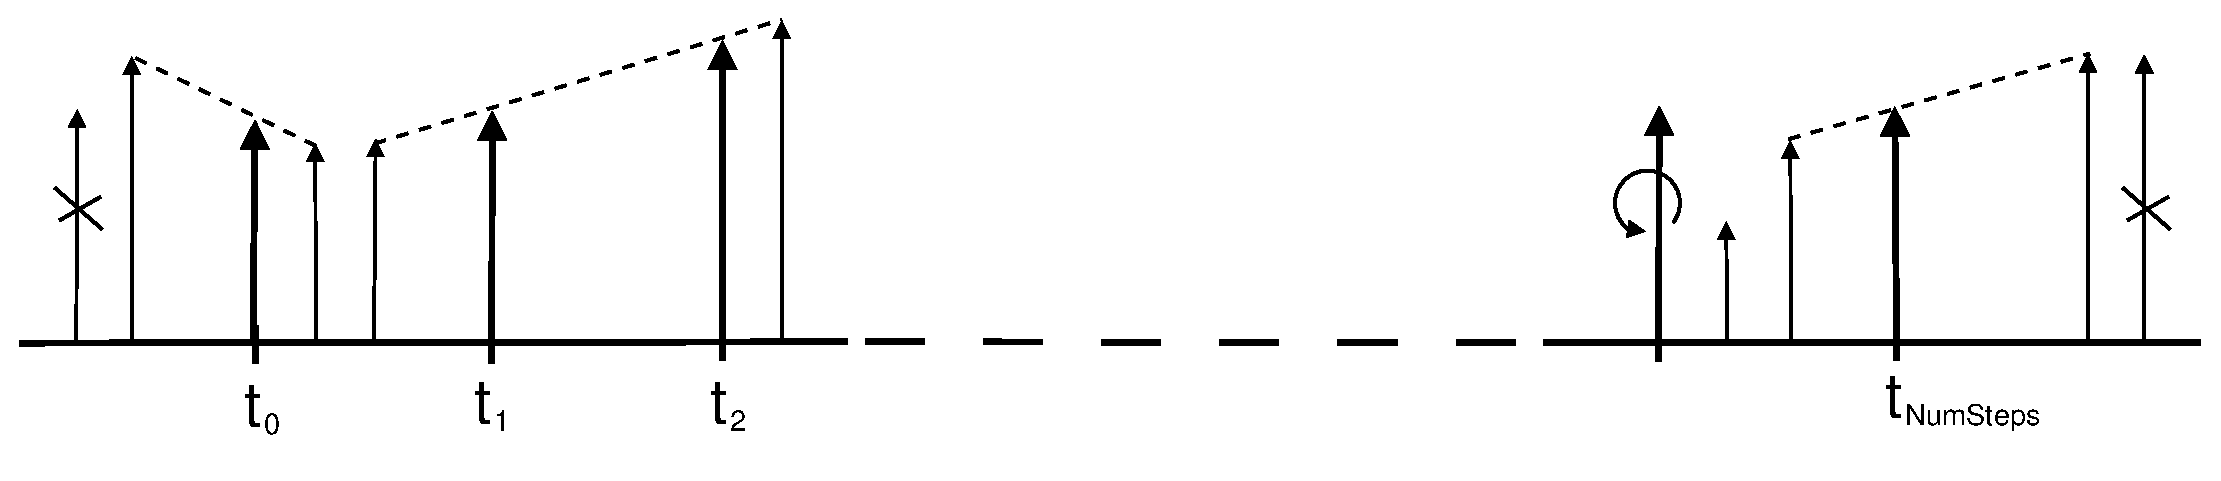
\includegraphics[width=10cm,angle=0]{./images/nettingmapping.eps}
\caption{Recovery mapping}
\label{timetranches}
\end{center}
\end{figure}

Veamos un ejemplo. Consideramos $\Upsilon_S(t_i,t_j)=1$ para no complicar los c\'alculos.
A la izquierda se representa el recovery original (sin estar mapeado a los nodos de
tiempo). A la derecha se encuentra el recovery mapeado a los nodos de tiempo.
\newline
\newline
\begin{minipage}[c]{0.4\columnwidth}%
\centering
\begin{tabular}{c|r}
\textbf{Date} & \textbf{Recovery} \\
\hline
17/04/2004 & -10.00 \\
           &        \\
           &        \\
05/01/2005 &   1.00 \\
20/01/2005 &   2.00 \\
           &        \\
15/03/2005 &   3.00 \\
           &        \\
           &        \\
30/08/2005 &   4.00 \\
           &        \\
15/12/2005 &   5.00 \\
25/12/2005 &  10.00 \\
\end{tabular}
\end{minipage}%
\begin{minipage}[c]{0.6\columnwidth}%
\centering
\begin{tabular}{c|c|c}
\textbf{$t_i$} & \textbf{Date}  & \textbf{Recovery} \\
\hline
      &            &      \\
$t_0$ & 30/10/2004 & $-10.00 + (1+10) \cdot \frac{196}{263} =  -1.8$\\
$t_1$ & 30/12/2004 & $-10.00 + (1+10) \cdot \frac{196}{263} =  0.75$ \\
      &            &      \\
      &            &      \\
$t_2$ & 28/02/2005 & $2 + (3-2) \cdot \frac{39}{54} = 2.72$ \\
      &            &      \\
$t_3$ & 30/04/2005 & $3.00 + (4-3) \cdot \frac{46}{168} = 3.27$ \\
$t_4$ & 30/06/2005 & $3.00 + (4-3) \cdot \frac{107}{168} = 3.64$ \\
$t_5$ & 30/08/2005 & $4.00$ \\
$t_6$ & 30/10/2005 & $4.00 + (5-4) \cdot \frac{61}{107} = 4.57$ \\
      &            &      \\
      &            &      \\
\end{tabular}
\end{minipage}%

%---------------------------------------------------------------------------

\subsection{Prec\'alculo de las p\'erdidas}

Sea $t_0, t_1, t_2, \cdots, t_{NumSteps}$ la partici\'on de tiempo usada.
Precalculamos las p\'erdidas en $t_0, t_1, t_2, \cdots, t_{NumSteps}$, o sea,
suponiendo que los tiempos de fallido se dan en $t_0, t_1, t_2, \cdots, t_{NumSteps}$.

\begin{displaymath}
Losses_i =
\left(
  \sum_{t=t_i}^{\infty} \textrm{cashflow}(t) \cdot \Upsilon_S(t,t_{NumSteps}) 
\right) - W_i
\end{displaymath}

donde $\Upsilon_S(t_i,t_j)$ es el coeficiente de transporte entre $t_i$ y $t_j$
usando la curva spot $S$.

Veamos un ejemplo. Consideramos $\Upsilon_S(t_i,t_j)=1$ para no complicar los c\'alculos.
A la izquierda se representa el cashflow original (sin estar mapeado a los nodos de
tiempo). A la derecha se encuentra el mismo cashflow mapeado a los nodos de tiempo.
Se supone que $W_i=3$ en cualquier instante de tiempo.
\newline
\newline
\begin{minipage}[c]{0.4\columnwidth}%
\centering
\begin{tabular}{c|r}
\textbf{Date} & \textbf{Cashflow} \\
\hline
17/04/2004 & -10.00 \\
           &        \\
           &        \\
05/01/2005 &   1.00 \\
20/01/2005 &   2.00 \\
           &        \\
15/03/2005 &   3.00 \\
           &        \\
           &        \\
30/08/2005 &   4.00 \\
           &        \\
15/12/2005 &   5.00 \\
25/12/2005 &   5.00 \\
\end{tabular}
\end{minipage}%
\begin{minipage}[c]{0.6\columnwidth}%
\centering
\begin{tabular}{c|c|c}
\textbf{$t_i$} & \textbf{Date}  & \textbf{Cashflow} \\
\hline
      &            &           \\
$t_0$ & 30/10/2004 & 20.00 - 3.00 = 17.00 \\
$t_1$ & 30/12/2004 & 20.00 - 3.00 = 17.00 \\
      &            &       \\
      &            &       \\
$t_2$ & 28/02/2005 & 17.00 - 3.00 = 14.00 \\
      &            &       \\
$t_3$ & 30/04/2005 & 14.00 - 3.00 = 11.00 \\
$t_4$ & 30/06/2005 & 14.00 - 3.00 = 11.00 \\
$t_5$ & 30/08/2005 & 14.00 - 3.00 = 11.00 \\
$t_6$ & 30/10/2005 & 10.00 - 3.00 = 7.00 \\
      &            &       \\
      &            &       \\
\end{tabular}
\end{minipage}%

%---------------------------------------------------------------------------

\section{Paso 7. Simulaci\'on}

Cada simulaci\'on consiste en generar n\'umeros aleatorios
mediante la c\'opula, simular el tiempo de fallido de cada
cliente (mape\'andolos sobre $t_1, t_2, \cdots, t_{NumSteps}$ y
resto) y evaluar cada segmento de cada segmentaci\'on.
\newline
\newline
Una forma de acelerar la convergencia implementada en CreditCruncher,
es la metodolog\'ia \emph{antithetic}\index{Antithetic}. Esta consiste
usar cada generaci\'on de n\'umeros aleatorios (computacionalmente
costosa de generar) 2 veces. Sea $(u_1, u_2, \cdots, u_{NumClients})$
n\'umeros aleatorios entre $0$ y $1$ generados por la realizaci\'on
de una c\'opula gaussiana. Entonces la realizaci\'on
$\left(1-u_1, 1-u_2, \cdots, 1-u_{NumClients}\right)$ es equiprobable 
a la anterior.

\subsection{Generaci\'on de n\'umeros aleatorios}

Generamos una realizaci\'on de la c\'opula $Q$ usando los pasos 3-5
del apartado \ref{apendix:gaussiancopula}.
\newline
\newline
Si se usa metodolog\'ia antithetic, solamente se generan los n\'umeros
de las simulaciones pares. Los n\'umeros aleatorios usados en las simulaciones
impares son $\vec{1}$ menos los de la simulaci\'on anterior 

\subsection{Simulaci\'on del tiempo de fallido}

Sean $Q_i$ el componente $i$-esimo de las c\'opula simulada. El objetivo es
simular el tiempo de fallido del cliente $i$-esimo. Conocemos el rating del
cliente $i$ en $t_0$. Realizamos el m\'etodo expuesto en \ref{res:mttd} teniendo
en cuenta que el tiempo retornado por la inversa de la funci\'on de supervivencia
es un n\'umero con decimales que debe ser mapeado a un nodo de tiempo; mapeamos 
este valor (tiempo de fallido) al nodo de tiempo 
($t_1, t_2, \cdots, t_{NumSteps}, t_{NumSteps+1}$) mas cercano por la derecha. 
Por ejemplo, si el tiempo de fallido simulado es $3.2$ y los nodos de tiempo son 
$0$, $3$, $6$ y $9$, el valor se mapear\'a a $6$.

\subsection{Valoraci\'on del segmento}

Los pasos anteriores nos proporcionan el tiempo simulado de fallido
para cada cliente, $t_w^1, t_w^2, \cdots, t_w^{NumClients}$. Obtenemos 
las p\'erdidas de los elementos del segmento $j$ de la siguiente forma:
\begin{displaymath}
Z_j = \sum_{i \in \Omega_j}
\left\{
\begin{array}{ll}
0                & \quad \textrm{if } t_w^i > t_{NumSteps}    \cr
Losses_{t_w^i}^i & \quad \textrm{if } t_w^i \leq t_{NumSteps} \cr
\end{array}
\right\}
\end{displaymath}

%---------------------------------------------------------------------------

\section{Paso 8. Valoraci\'on del riesgo}

Despu\'es de realizar $N$ simulaciones se dispone de $N$ valores para cada
segmento. Disponemos de $z_1, z_2, \cdots, z_N$. Fijado un nivel de confianza 
$\alpha$ y un nivel de VAR de $x$, usamos las indicaciones de \ref{res:risk} 
para calcular el Expected Loss, la Desviaci\'on Est\'andar, el VAR y el TCE y sus 
correspondientes errores est\'andares.

\begin{figure}[!hb]
\begin{center}
\includegraphics[width=12cm,angle=0]{./images/report.eps}
\caption{Evoluci\'on de los estad\'isticos de riesgo}
\label{timetranches}
\end{center}
\end{figure}
